
\lhead[\chaptername~\thechapter]{\rightmark}


\rhead[\leftmark]{}


\lfoot[\thepage]{}


\cfoot{}


\rfoot[]{\thepage}


\chapter{Decentralized mapping of tree structured applications}


\section{Overview}

Though it is difficult to map real life applications using a decentralized
algorithm , it is possible for certain special types of data flow
generating applications. Streaming applications that can be represented
as a tree happen to be one of those. 

Weichslgartner et al\cite{Weichslgartner:2011:DDM:1999946.1999979}present
a novel application-driven and resource-aware mapping methodology
for tree-structured streaming applications onto NoCs. This includes
strategies for mapping the source of streaming applications (seed
point selection), as well as embedding strategies so that each process
autonomously embeds its own succeeding tasks. The proposed embedding
strategies only consider the local view of neighboring cells on the
NoC which allows to significantly reduce computation and monitoring
overhead. We discuss the facets of this idea in the chapter.


\section{Application to hardware map}

Using the ideas we discussed in section 4.2 , we need to develop 3
maps.

The APCG (application characterization graph) which is a characteristic
graph of the application to be run. The HG (hardware graph) , which
represents the available resources in the form of a graph. And finally
the CTG (communication task graph) that is created by getting a suitable
map of APCG on HG.

Our target would be to find a CTG that minimizes congestion levels
, increases utilization and thus gives better performance and QoS.

Since we are considering a small subset of universal set of APCGs
, more specifically the tree-structured ones, we have some added constraints
on the applications we support.

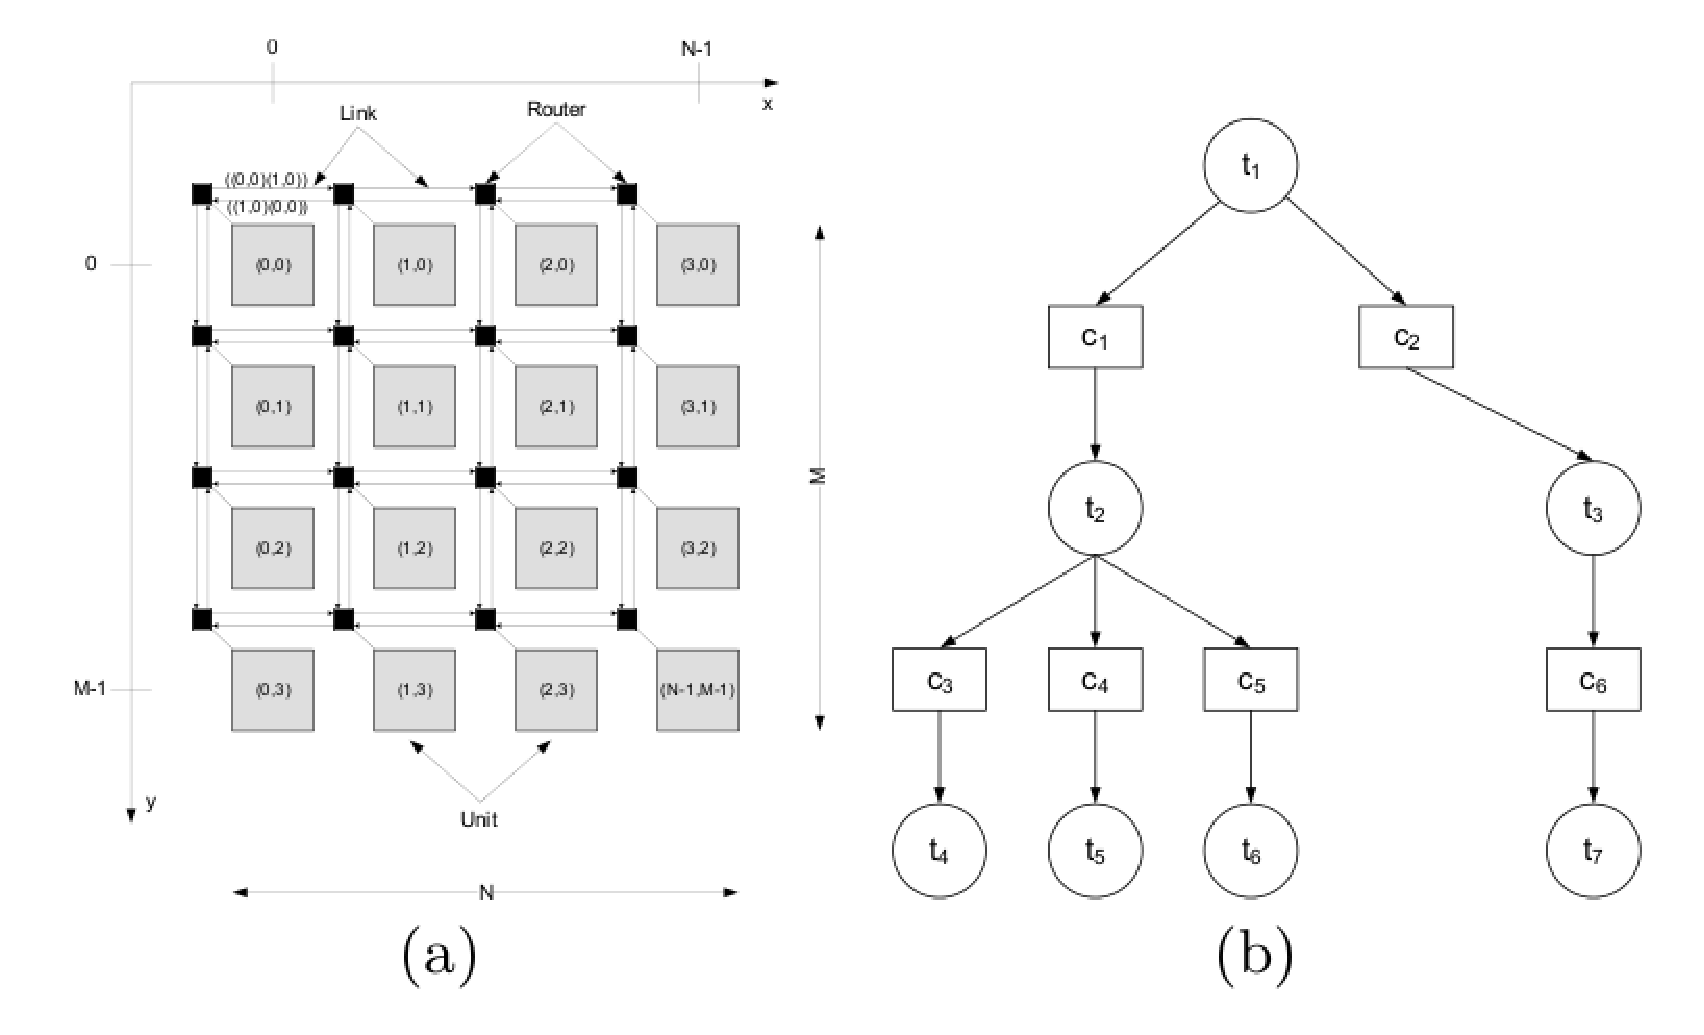
\includegraphics[width=10cm]{images/7}%
\framebox{\begin{minipage}[t]{0.2\columnwidth}%
Fig. 9\cite{Weichslgartner:2011:DDM:1999946.1999979}%
\end{minipage}}


\subsection{The APCG}

The methodology proposed in this paper is tailored for dataflow-dominated
streaming applications, with characteristics typically found in multimedia,
telecommunication, and signal processing. For the analysis presented
in this work, we make following assumptions:

A1: An application $i$ is executed periodically with period $P_{i}$
. 

A2: Data-dependencies between functional blocks result in a tree-shaped
dataflow. 

A3: Applications are characterized by bandwidth-oriented one-to-one
communications between tasks.

A graph-based, formal model of each applications as it is illustrated
in Fig. 9(b) can be given as follows: 

A tree-structured application $i$ is modeled as an acyclic bipartite
$G_{A}$($V_{i}$,$E_{i}$). The set $V_{i}=$$T_{i}+C_{i}$ is a
union of task vertices $T_{i}$and communication vertices $C_{i}$.
The application further satisfies the points discussed in section
4.2.


\subsection{The hardware graph}

HG - As is depicted in Fig 9(a) Each unit consists of one processing
element (PE) and one router that is connected to the local PE (through
a Network-Interface (NI)) and the four routers in the cardinal directions.
Tasks can be loaded and executed on the PEs. Each unit $u\in U$ provides
a limited amount of consumable resources that can be occupied by tasks,
e.g., memory for storing data and program code. This limit is denoted
as res(u). The maximal available bandwidth of a link $l\in L$ is
limited to band(l). 


\subsection{Creating the CTG}

Each task $t$$\in$ $T_{i}$ is characterized by its execution time
$exec(t,u)$ on PE $u\in U$ and the resources required for successfully
executing the task on the PE $req(t,u)$. Each message $c\in C$ is
designated with its payload $size(c)$. 

Once the CTG is created, we will be able to define values like bandwidth
of communication vertex $c$. 

$bw(c)=\frac{size(c)}{P_{i}}$

We will be further able to define values like load imposed by task
$t$ on unit $u$. 

$load(t,u)=\frac{exec(t,u)}{P_{i}}$

Application mapping can now be described as embedding the application
graph onto the NoC graph. This involves a) task mapping and b) communication
routing. Task mapping is denoted as m : $T_{i}$$\rightarrow U$ ,
i.e. , assigning tasks to processing elements. Routing is defined
as 

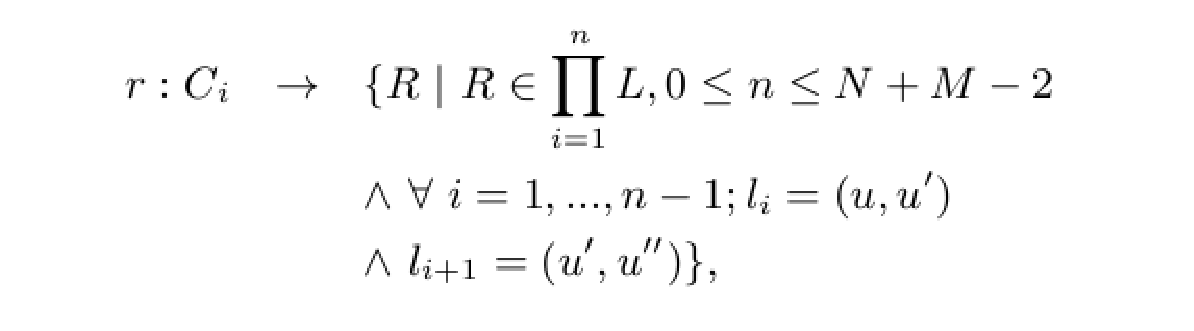
\includegraphics[width=9cm]{images/8}

i.e., each communication node is assigned with a route through communication
links. For example, a route with n hops can be described as a sequence
$r(c_{i})=(l_{1},l_{2}...l_{n})$. A feasible mapping is give, if
the following constraints hold:

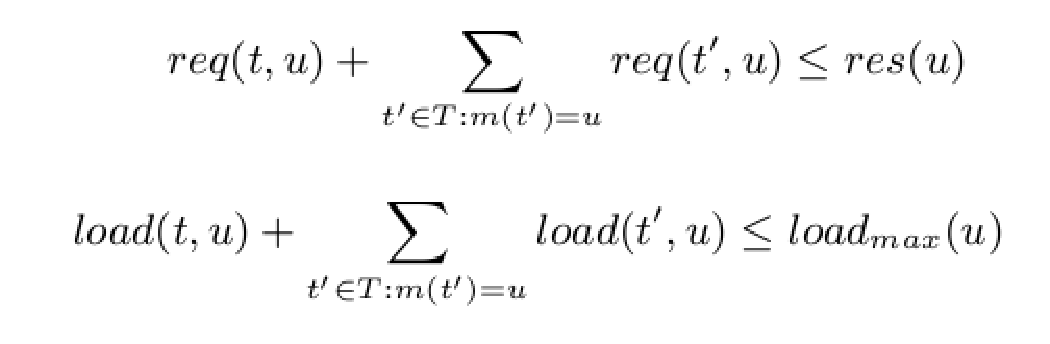
\includegraphics[width=7cm]{images/9}

where first equation ensures that resource restrictions are respected,
and second is the schedulability test of resource u. Moreover, a feasible
routing has to consider the available bandwidth.

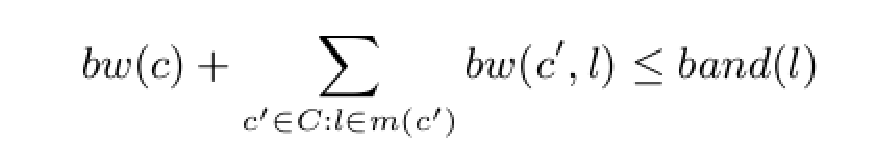
\includegraphics[width=7cm]{images/10}

\textbf{SELF-EMBEDDING ALGORITHM} - is the algorithm used in this
decentralized architecture. As the inspected application topologies
are treestructured, tasks can be embedded incrementally by an already
mapped predecessor task. Only the root nodes have to be placed differently,
since they have no predecessor tasks. There are various methods proposed
in \cite{Weichslgartner:2011:DDM:1999946.1999979} to select this
seed node. Distributing the mapping calculation to the task nodes
helps to parallelize the workload and to prevent a single point of
failure. 

A run example of the above algorithm:

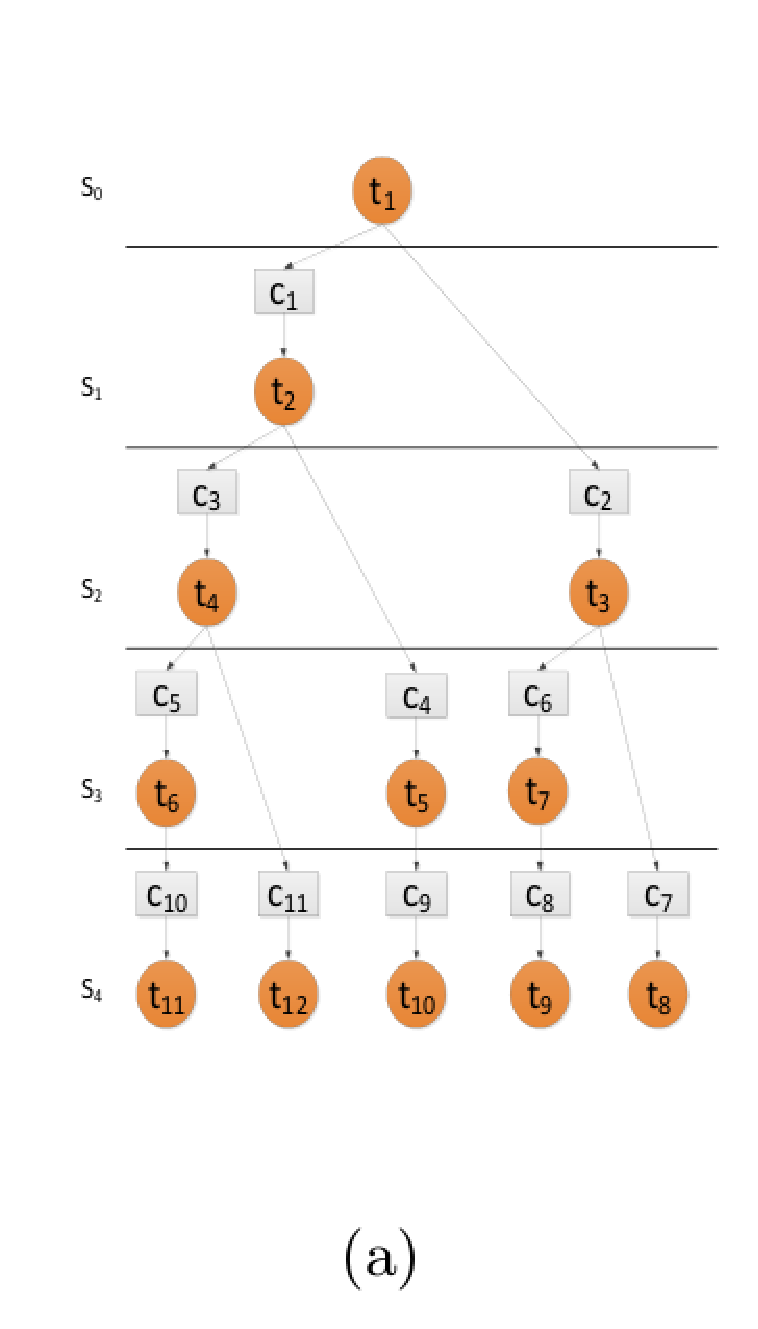
\includegraphics[height=10cm]{images/11}

\includegraphics[width=17cm]{images/12}

Figure 10: An example of a self-embedding algorithm with the initial
search space of 1 hop. In the upper half the search space is shown
and in the lower half the mapping. The root node t0 is embedded initial
with the seedpoint selection in mapping step S0 . In mapping step
S1 it starts the embedding algorithm for t2 and c1 . In S2 , it starts
the embedding for t3 and c2 . In the same mapping step, t2 itself
can start the embedding of t4 and c3 , and so on. While embedding
the right successor, the already mapped left successor can embed its
own successors in parallel. 

\ \\

\textbf{SEED POINT SELECTION} 

As every task places its succeeding tasks and communication, the initial
task or root task has to be placed by a different algorithm. For these
tasks, it is necessary to find those units on the NoC on which it
is suitable to load the root nodes. We call these units seed points
($U_{s}$) and several methodologies are available to determine this
set. As we don\textquoteright{}t want to loose the decentralized characteristics
of our approach, the seed point determination should not have a global
view of the entire NoC system. Nevertheless, some global information,
like the size of NoC, previous seed points and cluster information
have to be stored centrally. However, these algorithms are only executed
once per application and the saved information is linear in the NoC
size. So the scalability is kept. 

\textbf{SIMULATION RESULTS}

Authors of the above cited paper have run elaborate simulations and
found that for specific structures (in this case , tree structured
applications), the decentralized algorithms for mapping give results
at par with the centralized ones.


\chapter{Conclusion}

In this report we discussed the various paradigms available for running
real life applications on the NoC architectures. We analysed the reasons
that forced us to make the switch from the currently prevalent architectures.
We established the asymptotic supremacy of NoCs over other architectures.
We saw that the applications need to be mapped before being run on
a multicore. Amongst the various paradigms used for mapping centralized
has been deeply explored till date whereas decentralized has been
ignored for a while. We reasoned that the centralized approach is
not scalable , and that going decentralized is the best way for future.
The recent paper about decentralized mapping of tree structured applications
has shown that with sufficient attention , decentralized mapping mechanisms
can come at par with the centralized ones , thus paving way for a
scalable technology.
